\documentclass[12pt]{article}                             
\usepackage[utf8]{inputenc}                               
\usepackage[russian]{babel}                               
\usepackage{geometry}                                     
\usepackage{amsmath}                                      
\geometry{a4paper}                                        
\usepackage{graphicx}                                     
\begin{document}                                          
\begin{titlepage}                                         
	\begin{center}                                          
		\Huge                                                 
		Сан-Юрьевич                                            
		\vspace*{1cm}                                         
                                                           
		\textbf{Дифференциальный зачёт}                       
                                                           
		\vspace{0.5cm}                                        
		\vspace{1.5cm}                                        
		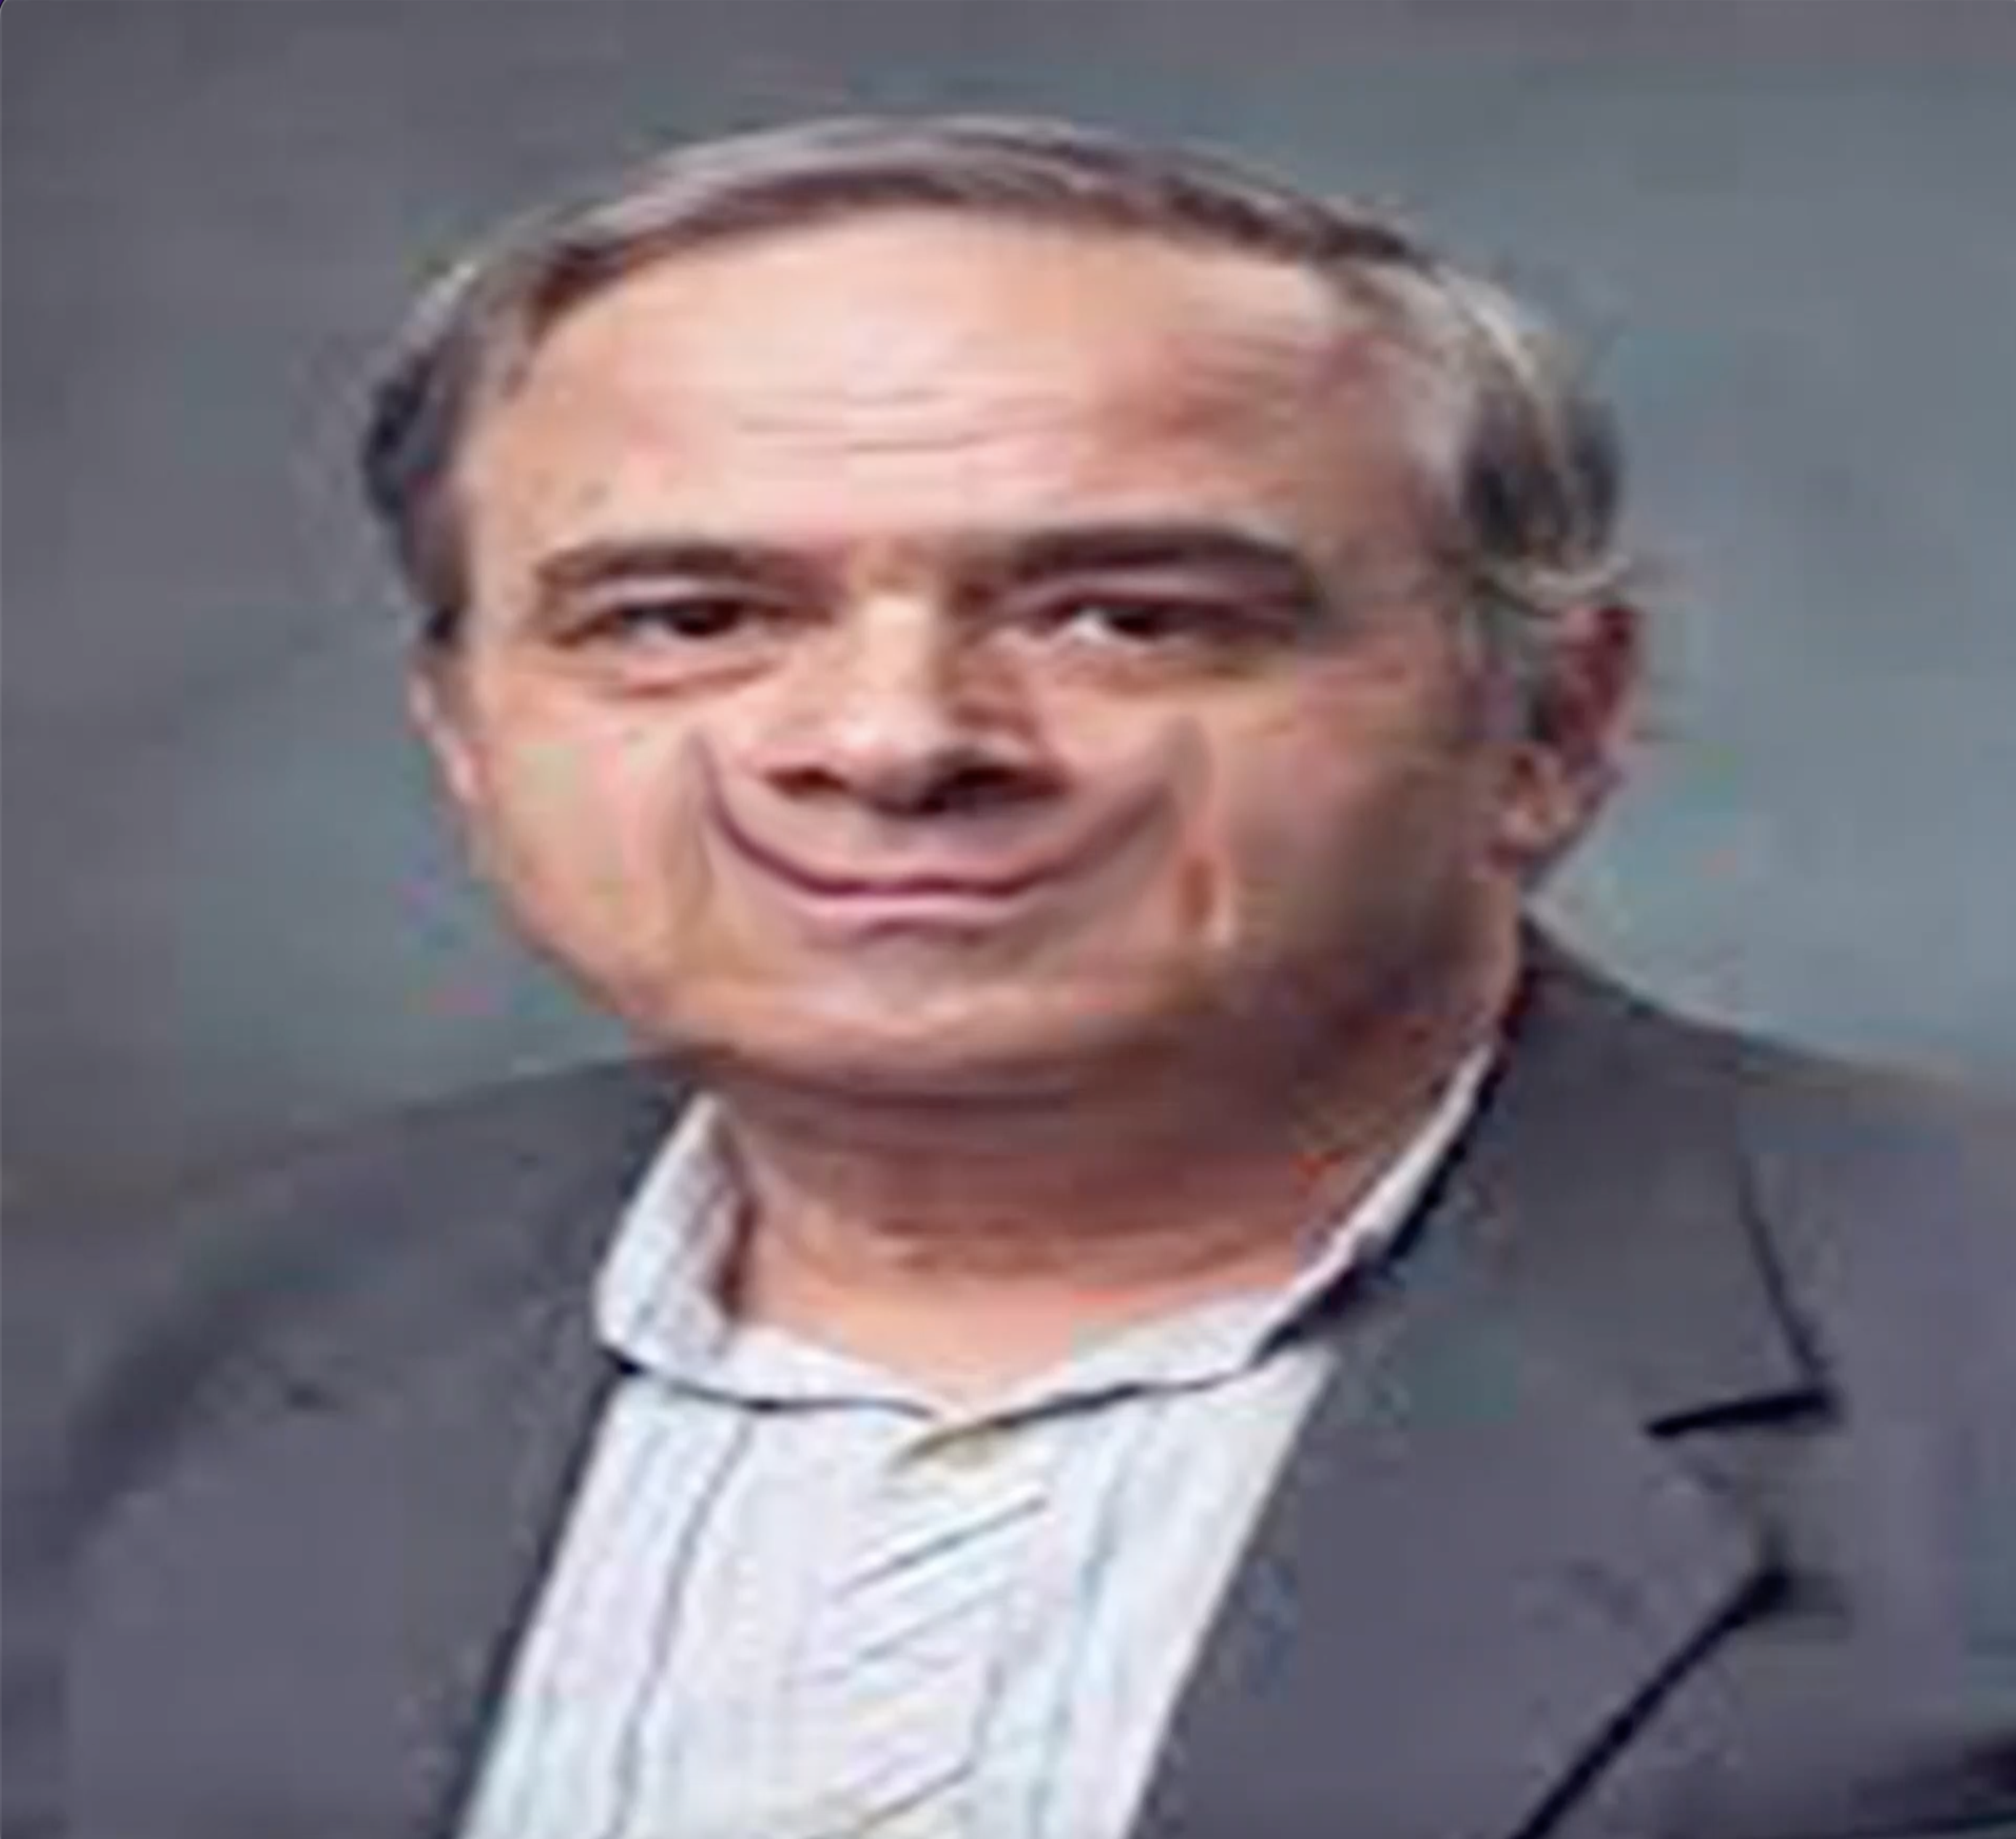
\includegraphics[width = 10 cm]{imgs/petrovich.png}   
		\begin{minipage}{10cm}                                
		\vspace*{2cm}                                         
			\begin{center}                                      
				Из МФТИ, с любовью                                 
			\end{center}                                        
		
\includegraphics[width = 3 cm]{imgs/with_love.png}    
		\end{minipage}                                        
                                                           
	\end{center}                                            
\end{titlepage}                                           
\newpage                                                  
\Huge                                                     
	Посчитаем производную\\                                
\newline                                                  
\normalfont                                               
\normalsize                                               
А Флуктуационно-диссипационная теорема гласит, что:  \begin{equation}
	\frac{\partial}{\partial x}\left( \sin {x^{2}}\right) 
\end{equation}
Очевидно, что по критерию Сильвестра:  \begin{equation}
	\frac{\partial}{\partial x}\left( x^{2}\right) \cdot \cos {x^{2}}
\end{equation}
Слава Украине, героям слава:  \begin{equation}
	\frac{\partial}{\partial x}\left( x\right) \cdot 2\cdot x^{2 - 1}\cdot \cos {x^{2}}
\end{equation}
А по теореме Лиувилля об интеграле уравнения Гамильтона — Якоби:  \begin{equation}
	1\cdot 2\cdot x^{2 - 1}\cdot \cos {x^{2}}
\end{equation}
Предлагаем читателю убедиться в том, что конечный ответ: 
\begin{equation}
	2\cdot x\cdot \cos {x^{2}}
\end{equation}
\end{document}
